\section*{CHƯƠNG 2. TÌM HIỂU VÀ PHÂN TÍCH HỆ THỐNG}
\setcounter{section}{2}
\setcounter{subsection}{0} %LƯU Ý MỖI LẦN THÊM CHƯƠNG MỚI CẦN THÊM CÂU NÀY ĐỂ RESET THỨ TỰ CỦA SUBSECTON VỀ 1
\setcounter{table}{0} % LƯU Ý SAU MỖI LẦN GỌI BẢNG HAY HÌNH ẢNH PHẢI THÊM CÂU NÀY ĐỂ RESET THỨ TỰ
\setcounter{figure}{0} %% LƯU Ý SAU MỖI LẦN GỌI BẢNG HAY HÌNH ẢNH PHẢI THÊM CÂU NÀY ĐỂ RESET THỨ TỰ
\addcontentsline{toc}{section}{\numberline{}CHƯƠNG 2. PHÂN TÍCH HỆ THỐNG}
Chương này trình bày chi tiết quá trình phân tích hệ thống, dựa trên các yêu cầu đã được xác định trong Phần mở đầu và Chương 1. Nội dung bao gồm các bước sau:\begin{adjustwidth}{1.5em}{}
	\begin{itemize}
		\item Thiết kế các thẻ CRC (Class - Responsibility - Collaboration Card) cùng các lớp dựa trên thông tin thu thập từ các sơ đồ use case mô tả chức năng của hệ thống.
		\item Xây dựng sơ đồ lớp với đầy đủ thuộc tính và phương thức, dựa trên các lớp đã được định nghĩa.
		\item Sau khi xác định thuộc tính, phương thức và chức năng của các lớp, tiếp tục thiết kế sơ đồ tuần tự để minh họa chi tiết sự tương tác giữa các lớp khi thực hiện các chức năng cụ thể.
	\end{itemize}
\end{adjustwidth}
% \newpage
\subsection{Thẻ CRC (Class - Responsibility - Collaboration Card)}

\subsubsection{Thẻ CRC lớp Tài khoản người dùng}

\begin{xltabular}{\textwidth}{
		>{\centering\arraybackslash}X
	}
	\caption{\bfseries \fontsize{12pt}{0pt}\selectfont Thẻ CRC lớp Tài khoản người dùng}
	\\
	\begin{tabularx}{0.9\textwidth}{X}
		Mặt trước thẻ
	\end{tabularx}
	\begin{tabularx}{0.9\textwidth}{|X|X|}
		\hline
		\textbf{Tên lớp:} Tài khoản (account)                                     & \textbf{ID:} 0                                                                                           \\
		\hline
		\textbf{Mô tả:} Lớp quản lý thông tin tài khoản người dùng trong hệ thống & \textbf{Use case liên quan:}  Đăng ký tài khoản, Quản lý tài khoản cá nhân, Quản lí thông tin người dùng \\
		\hline
		\textbf{Trách nhiệm (Responsibility):}                                    & \textbf{Các lớp cộng tác (Collaboration):}                                                               \\
		Xử lý đăng nhập và đăng xuất

		Đăng ký tài khoản mới cho người dùng
		                                                                          &
		Token đăng nhập

		Người dùng
		\\
		\hline
	\end{tabularx}
	\\
	\begin{tabularx}{0.9\textwidth}{X}
		Mặt sau thẻ
	\end{tabularx}
	\begin{tabularx}{0.9\textwidth}{|X|X|}
		\hline
		\textbf{Thuộc tính (Attributes):} & \\
		id(uuid)

		email(string)

		password(string)
		                                  &
		role(integer)

		createdAt(Datetime)

		updatedAt(Datetime)
		\\ \hline
	\end{tabularx}
	\\
	\begin{tabularx}{0.9\textwidth}{|X|}
		\hline
		\textbf{Mối quan hệ (Relationships)} \\
		Tổng quát hóa (Generalize):

		Toàn thể - Bộ phận (Aggregation):

		Liên kết (Association): Token đăng nhập, Người dùng
		\\
		\hline
	\end{tabularx}
\end{xltabular}

\subsubsection{Thẻ CRC lớp Token}

\begin{xltabular}{\textwidth}{
		>{\centering\arraybackslash}X
	}
	\caption{\bfseries \fontsize{12pt}{0pt}\selectfont Thẻ CRC lớp Token}
	\\
	\begin{tabularx}{0.9\textwidth}{X}
		Mặt trước thẻ
	\end{tabularx}
	\begin{tabularx}{0.9\textwidth}{|X|X|}
		\hline
		\textbf{Tên lớp:} Token                                                           & \textbf{ID:} 1                                     \\
		\hline
		\textbf{Mô tả:} Lớp quản lý thông tin token liên kết với mỗi tài khoản người dùng & \textbf{Use case liên quan:}  Đăng nhập, đăng xuất \\
		\hline
		\textbf{Trách nhiệm (Responsibility):}                                            & \textbf{Các lớp cộng tác (Collaboration):}         \\
		Quản lý vòng đời của access\_token và refresh\_token (tạo mới, xóa khi cần)

		Xác minh token để kiểm tra tính hợp lệ trong các yêu cầu của người dùng

		Đảm bảo tính hợp lệ của phiên đăng nhập
		                                                                                  &
		Tài khoản người dùng
		\\
		\hline
	\end{tabularx}
	\\
	\begin{tabularx}{0.9\textwidth}{X}
		Mặt sau thẻ
	\end{tabularx}
	\begin{tabularx}{0.9\textwidth}{|X|X|}
		\hline
		\textbf{Thuộc tính (Attributes):} & \\
		id(uuid)

		account\_id(string)

		refresh\_token(string)

		expired\_At(Datetime)
		                                  &
		is\_expired(integer)

		createdAt(Datetime)

		updatedAt(Datetime)
		\\ \hline
	\end{tabularx}
	\\
	\begin{tabularx}{0.9\textwidth}{|X|}
		\hline
		\textbf{Mối quan hệ (Relationships)} \\
		Tổng quát hóa (Generalize):

		Toàn thể - Bộ phận (Aggregation):

		Liên kết (Association): Tài khoản người dùng
		\\
		\hline
	\end{tabularx}
\end{xltabular}

\subsubsection{Thẻ CRC lớp Vai trò người dùng}

\begin{xltabular}{\textwidth}{
		>{\centering\arraybackslash}X
	}
	\caption{\bfseries \fontsize{12pt}{0pt}\selectfont Thẻ CRC lớp Vai trò người dùng}
	\\
	\begin{tabularx}{0.9\textwidth}{X}
		Mặt trước thẻ
	\end{tabularx}
	\begin{tabularx}{0.9\textwidth}{|X|X|}
		\hline
		\textbf{Tên lớp:} Vai trò người dùng (user\_role)                               & \textbf{ID:} 2                                             \\
		\hline
		\textbf{Mô tả:} Lớp quản lý thông tin các vai trò của người dùng trong hệ thống & \textbf{Use case liên quan:}  Quản lí thông tin người dùng \\
		\hline
		\textbf{Trách nhiệm (Responsibility):}                                          & \textbf{Các lớp cộng tác (Collaboration):}                 \\
		Lưu trữ và quản lý các vai trò người dùng (như Bệnh nhân, Bác sĩ, Quản trị viên)

		Cung cấp thông tin vai trò để phân quyền truy cập trong hệ thống
		                                                                                &
		Người dùng
		\\
		\hline
	\end{tabularx}
	\\
	\begin{tabularx}{0.9\textwidth}{X}
		Mặt sau thẻ
	\end{tabularx}
	\begin{tabularx}{0.9\textwidth}{|X|X|}
		\hline
		\textbf{Thuộc tính (Attributes):} & \\
		id(uuid)

		role\_name(string)
		                                  &
		createdAt(Datetime)

		updatedAt(Datetime)
		\\ \hline
	\end{tabularx}
	\\
	\begin{tabularx}{0.9\textwidth}{|X|}
		\hline
		\textbf{Mối quan hệ (Relationships)} \\
		Tổng quát hóa (Generalize):

		Toàn thể - Bộ phận (Aggregation):

		Liên kết (Association): Người dùng
		\\
		\hline
	\end{tabularx}
\end{xltabular}

\subsubsection{Thẻ CRC lớp Trạng thái người dùng}

\begin{xltabular}{\textwidth}{
		>{\centering\arraybackslash}X
	}
	\caption{\bfseries \fontsize{12pt}{0pt}\selectfont Thẻ CRC lớp Trạng thái người dùng}
	\\
	\begin{tabularx}{0.9\textwidth}{X}
		Mặt trước thẻ
	\end{tabularx}
	\begin{tabularx}{0.9\textwidth}{|X|X|}
		\hline
		\textbf{Tên lớp:} Trạng thái người dùng (user\_status)                             & \textbf{ID:} 3                                             \\
		\hline
		\textbf{Mô tả:} Lớp quản lý thông tin các trạng thái của người dùng trong hệ thống & \textbf{Use case liên quan:}  Quản lí thông tin người dùng \\
		\hline
		\textbf{Trách nhiệm (Responsibility):}                                             & \textbf{Các lớp cộng tác (Collaboration):}                 \\
		Lưu trữ các trạng thái hoạt động của người dùng (ví dụ: hoạt động, bị khóa, tạm ngưng)

		Cung cấp thông tin trạng thái để hỗ trợ quản lý quyền truy cập hệ thống
		                                                                                   &
		Người dùng
		\\
		\hline
	\end{tabularx}
	\\
	\begin{tabularx}{0.9\textwidth}{X}
		Mặt sau thẻ
	\end{tabularx}
	\begin{tabularx}{0.9\textwidth}{|X|X|}
		\hline
		\textbf{Thuộc tính (Attributes):} & \\
		id(uuid)

		status\_description(string)
		                                  &
		createdAt(Datetime)

		updatedAt(Datetime)
		\\ \hline
	\end{tabularx}
	\\
	\begin{tabularx}{0.9\textwidth}{|X|}
		\hline
		\textbf{Mối quan hệ (Relationships)} \\
		Tổng quát hóa (Generalize):

		Toàn thể - Bộ phận (Aggregation):

		Liên kết (Association): Người dùng
		\\
		\hline
	\end{tabularx}
\end{xltabular}

\subsubsection{Thẻ CRC lớp Người dùng}

\begin{xltabular}{\textwidth}{
		>{\centering\arraybackslash}X
	}
	\caption{\bfseries \fontsize{12pt}{0pt}\selectfont Thẻ CRC lớp Người dùng}
	\\
	\begin{tabularx}{0.9\textwidth}{X}
		Mặt trước thẻ
	\end{tabularx}
	\begin{tabularx}{0.9\textwidth}{|X|X|}
		\hline
		\textbf{Tên lớp:} Người dùng (User)                                                      & \textbf{ID:} 4                                                                               \\
		\hline
		\textbf{Mô tả:} Lớp quản lý thông tin cá nhân và quyền hạn của người dùng trong hệ thống & \textbf{Use case liên quan:}  Đăng ký tài khoản, Quản lý tài khoản cá nhân, Quản lý lịch hẹn \\
		\hline
		\textbf{Trách nhiệm (Responsibility):}                                                   & \textbf{Các lớp cộng tác (Collaboration):}                                                   \\
		Quản lý thông tin người dùng, bao gồm thêm mới, chỉnh sửa và xóa dữ liệu

		Truy vấn danh sách người dùng hiện có trong hệ thống dựa trên các tiêu chí như ID, tài khoản, hoặc vai trò
		                                                                                         &
		Tài khoản
		\\
		\hline
	\end{tabularx}
	\\
	\begin{tabularx}{0.9\textwidth}{X}
		Mặt sau thẻ
	\end{tabularx}
	\begin{tabularx}{0.9\textwidth}{|X|X|}
		\hline
		\textbf{Thuộc tính (Attributes):} & \\
		id(uuid)

		username(string)

		birth(timestamps)

		phone\_number(string)
		                                  &
		image(string)

		role(integer)

		createdAt(Datetime)

		updatedAt(Datetime)
		\\ \hline
	\end{tabularx}
	\\
	\begin{tabularx}{0.9\textwidth}{|X|}
		\hline
		\textbf{Mối quan hệ (Relationships)} \\
		Tổng quát hóa (Generalize):

		Toàn thể - Bộ phận (Aggregation):

		Liên kết (Association): Tài khoản, Vai trò người dùng, Trạng thái người dùng, Lịch hẹn, Thiết bị, Dữ liệu phiên đo
		\\
		\hline
	\end{tabularx}
\end{xltabular}

\subsubsection{Thẻ CRC lớp Loại thiết bị}

\begin{xltabular}{\textwidth}{
		>{\centering\arraybackslash}X
	}
	\caption{\bfseries \fontsize{12pt}{0pt}\selectfont Thẻ CRC lớp Loại thiết bị}
	\\
	\begin{tabularx}{0.9\textwidth}{X}
		Mặt trước thẻ
	\end{tabularx}
	\begin{tabularx}{0.9\textwidth}{|X|X|}
		\hline
		\textbf{Tên lớp:} Loại thiết bị (device\_type)                                      & \textbf{ID:} 5                                 \\
		\hline
		\textbf{Mô tả:} Lớp quản lý thông tin các loại thiết bị được sử dụng trong hệ thống & \textbf{Use case liên quan:}  Quản lí thiết bị \\
		\hline
		\textbf{Trách nhiệm (Responsibility):}                                              & \textbf{Các lớp cộng tác (Collaboration):}     \\
		Lưu trữ và quản lý danh sách các loại thiết bị
		                                                                                    &
		Thiết bị
		\\
		\hline
	\end{tabularx}
	\\
	\begin{tabularx}{0.9\textwidth}{X}
		Mặt sau thẻ
	\end{tabularx}
	\begin{tabularx}{0.9\textwidth}{|X|X|}
		\hline
		\textbf{Thuộc tính (Attributes):} & \\
		id(uuid)

		type\_name(string)
		                                  &
		createdAt(Datetime)

		updatedAt(Datetime)
		\\ \hline
	\end{tabularx}
	\\
	\begin{tabularx}{0.9\textwidth}{|X|}
		\hline
		\textbf{Mối quan hệ (Relationships)} \\
		Tổng quát hóa (Generalize):

		Toàn thể - Bộ phận (Aggregation):

		Liên kết (Association): Thiết bị
		\\
		\hline
	\end{tabularx}
\end{xltabular}

\subsubsection{Thẻ CRC lớp Trạng thái thiết bị}

\begin{xltabular}{\textwidth}{
		>{\centering\arraybackslash}X
	}
	\caption{\bfseries \fontsize{12pt}{0pt}\selectfont Thẻ CRC lớp Trạng thái thiết bị}
	\\
	\begin{tabularx}{0.9\textwidth}{X}
		Mặt trước thẻ
	\end{tabularx}
	\begin{tabularx}{0.9\textwidth}{|X|X|}
		\hline
		\textbf{Tên lớp:} Trạng thái thiết bị (device\_status)                                        & \textbf{ID:} 6                                 \\
		\hline
		\textbf{Mô tả:} Lớp quản lý thông tin các trạng thái của thiết bị được sử dụng trong hệ thống & \textbf{Use case liên quan:}  Quản lí thiết bị \\
		\hline
		\textbf{Trách nhiệm (Responsibility):}                                                        & \textbf{Các lớp cộng tác (Collaboration):}     \\
		Lưu trữ danh sách các trạng thái của thiết bị (ví dụ: Hoạt động, Không hoạt động, Bảo trì)

		Cung cấp thông tin trạng thái cho các chức năng quản lý và phân công thiết bị
		                                                                                              &
		Thiết bị
		\\
		\hline
	\end{tabularx}
	\\
	\begin{tabularx}{0.9\textwidth}{X}
		Mặt sau thẻ
	\end{tabularx}
	\begin{tabularx}{0.9\textwidth}{|X|X|}
		\hline
		\textbf{Thuộc tính (Attributes):} & \\
		id(uuid)

		status\_description(string)
		                                  &
		createdAt(Datetime)

		updatedAt(Datetime)
		\\ \hline
	\end{tabularx}
	\\
	\begin{tabularx}{0.9\textwidth}{|X|}
		\hline
		\textbf{Mối quan hệ (Relationships)} \\
		Tổng quát hóa (Generalize):

		Toàn thể - Bộ phận (Aggregation):

		Liên kết (Association): Thiết bị
		\\
		\hline
	\end{tabularx}
\end{xltabular}

\subsubsection{Thẻ CRC lớp Thiết bị}

\begin{xltabular}{\textwidth}{
		>{\centering\arraybackslash}X
	}
	\caption{\bfseries \fontsize{12pt}{0pt}\selectfont Thẻ CRC lớp Thiết bị}
	\\
	\begin{tabularx}{0.9\textwidth}{X}
		Mặt trước thẻ
	\end{tabularx}
	\begin{tabularx}{0.9\textwidth}{|X|X|}
		\hline
		\textbf{Tên lớp:} Thiết bị (device)                                                     & \textbf{ID:} 7                                 \\
		\hline
		\textbf{Mô tả:} Lớp quản lý thông tin chi tiết các thiết bị được sử dụng trong hệ thống & \textbf{Use case liên quan:}  Quản lí thiết bị \\
		\hline
		\textbf{Trách nhiệm (Responsibility):}                                                  & \textbf{Các lớp cộng tác (Collaboration):}     \\
		Quản lý thông tin thiết bị: thêm mới, chỉnh sửa, và xóa dữ liệu thiết bị

		Truy vấn danh sách các thiết bị hiện có trong hệ thống dựa trên các tiêu chí như ID bệnh nhân và bác sĩ
		                                                                                        &
		Thiết bị
		\\
		\hline
	\end{tabularx}
	\\
	\begin{tabularx}{0.9\textwidth}{X}
		Mặt sau thẻ
	\end{tabularx}
	\begin{tabularx}{0.9\textwidth}{|X|X|}
		\hline
		\textbf{Thuộc tính (Attributes):} & \\
		id(uuid)

		user\_id(string)

		device\_name(string)

		information(string)

		device\_type\_id(integer)
		                                  &
		status\_id(integer)

		start\_time(timestamps)

		end\_time(timestamps)

		createdAt(Datetime)

		updatedAt(Datetime)
		\\ \hline
	\end{tabularx}
	\\
	\begin{tabularx}{0.9\textwidth}{|X|}
		\hline
		\textbf{Mối quan hệ (Relationships)} \\
		Tổng quát hóa (Generalize):

		Toàn thể - Bộ phận (Aggregation):

		Liên kết (Association): Dữ liệu phiên đo, Người dùng, Loại thiết bị, Trạng thái thiết bị, Thông tin chi tiết thiết bị
		\\
		\hline
	\end{tabularx}
\end{xltabular}

\subsubsection{Thẻ CRC lớp Thông số kỹ thuật}

\begin{xltabular}{\textwidth}{
		>{\centering\arraybackslash}X
	}
	\caption{\bfseries \fontsize{12pt}{0pt}\selectfont Thẻ CRC lớp Thông số kỹ thuật}
	\\
	\begin{tabularx}{0.9\textwidth}{X}
		Mặt trước thẻ
	\end{tabularx}
	\begin{tabularx}{0.9\textwidth}{|X|X|}
		\hline
		\textbf{Tên lớp:} Thông số kỹ thuật (device\_details)                                                         & \textbf{ID:} 8                                 \\
		\hline
		\textbf{Mô tả:} Lớp quản lý thông tin chi tiết thông số kỹ thuật của các thiết bị được sử dụng trong hệ thống & \textbf{Use case liên quan:}  Quản lí thiết bị \\
		\hline
		\textbf{Trách nhiệm (Responsibility):}                                                                        & \textbf{Các lớp cộng tác (Collaboration):}     \\
		Lưu trữ và quản lý thông số kỹ thuật của thiết bị: thêm mới, chỉnh sửa, và xóa thông số theo ID thiết bị

		Truy vấn các thông số kỹ thuật dựa trên ID thiết bị cụ thể
		                                                                                                              &
		Thiết bị
		\\
		\hline
	\end{tabularx}
	\\
	\begin{tabularx}{0.9\textwidth}{X}
		Mặt sau thẻ
	\end{tabularx}
	\begin{tabularx}{0.9\textwidth}{|X|X|}
		\hline
		\textbf{Thuộc tính (Attributes):} & \\
		id(uuid)

		device\_id(string)

		detail\_name(string)

		detail\_type(integer)
		                                  &
		value(string)

		information(string)

		createdAt(Datetime)

		updatedAt(Datetime)
		\\ \hline
	\end{tabularx}
	\\
	\begin{tabularx}{0.9\textwidth}{|X|}
		\hline
		\textbf{Mối quan hệ (Relationships)} \\
		Tổng quát hóa (Generalize):

		Toàn thể - Bộ phận (Aggregation):

		Liên kết (Association): Thiết bị
		\\
		\hline
	\end{tabularx}
\end{xltabular}

\subsubsection{Thẻ CRC lớp Dữ liệu phiên đo}

\begin{xltabular}{\textwidth}{
		>{\centering\arraybackslash}X
	}
	\caption{\bfseries \fontsize{12pt}{0pt}\selectfont Thẻ CRC lớp Dữ liệu phiên đo}
	\\
	\begin{tabularx}{0.9\textwidth}{X}
		Mặt trước thẻ
	\end{tabularx}
	\begin{tabularx}{0.9\textwidth}{|X|X|}
		\hline
		\textbf{Tên lớp:} Dữ liệu phiên đo (records)                                & \textbf{ID:} 9                                         \\
		\hline
		\textbf{Mô tả:} Lớp quản lý thông tin các Dữ liệu phiên đo của mỗi phiên đo & \textbf{Use case liên quan:}  Quản lý dữ liệu phiên đo \\
		\hline
		\textbf{Trách nhiệm (Responsibility):}                                      & \textbf{Các lớp cộng tác (Collaboration):}             \\
		Lưu trữ và quản lý danh sách các dữ liệu phiên đo: chỉnh sửa, và xóa dữ liệu

		Truy vấn danh sách dữ liệu phiên đo dựa trên ID bệnh nhân hoặc ID bác sĩ
		                                                                            &
		Người dùng

		Thiết bị
		\\
		\hline
	\end{tabularx}
	\\
	\begin{tabularx}{0.9\textwidth}{X}
		Mặt sau thẻ
	\end{tabularx}
	\begin{tabularx}{0.9\textwidth}{|X|X|}
		\hline
		\textbf{Thuộc tính (Attributes):} & \\
		id(uuid)

		patient\_id(string)

		device\_id(string)

		data\_rec\_url(string)
		                                  &
		start\_time(string)

		end\_time(string)

		createdAt(Datetime)

		updatedAt(Datetime)
		\\ \hline
	\end{tabularx}
	\\
	\begin{tabularx}{0.9\textwidth}{|X|}
		\hline
		\textbf{Mối quan hệ (Relationships)} \\
		Tổng quát hóa (Generalize):

		Toàn thể - Bộ phận (Aggregation):

		Liên kết (Association): Thiết bị, Người dùng
		\\
		\hline
	\end{tabularx}
\end{xltabular}

\subsubsection{Thẻ CRC lớp Loại lịch hẹn}

\begin{xltabular}{\textwidth}{
		>{\centering\arraybackslash}X
	}
	\caption{\bfseries \fontsize{12pt}{0pt}\selectfont Thẻ CRC lớp Loại lịch hẹn}
	\\
	\begin{tabularx}{0.9\textwidth}{X}
		Mặt trước thẻ
	\end{tabularx}
	\begin{tabularx}{0.9\textwidth}{|X|X|}
		\hline
		\textbf{Tên lớp:} Loại lịch hẹn (schedule\_type)                   & \textbf{ID:} 10                                \\
		\hline
		\textbf{Mô tả:} Lớp quản lý thông tin các loại lịch hẹn có thể đặt & \textbf{Use case liên quan:}  Quản lý lịch hẹn \\
		\hline
		\textbf{Trách nhiệm (Responsibility):}                             & \textbf{Các lớp cộng tác (Collaboration):}     \\
		Lưu trữ danh sách các loại lịch hẹn khả dụng (ví dụ: Lịch khám, Lịch tư vấn thiết bị)

		Cung cấp thông tin các loại lịch hẹn cho các chức năng liên quan đến lập lịch
		                                                                   &
		Lịch hẹn
		\\
		\hline
	\end{tabularx}
	\\
	\begin{tabularx}{0.9\textwidth}{X}
		Mặt sau thẻ
	\end{tabularx}
	\begin{tabularx}{0.9\textwidth}{|X|X|}
		\hline
		\textbf{Thuộc tính (Attributes):} & \\
		id(uuid)

		type\_name(string)
		                                  &
		createdAt(Datetime)

		updatedAt(Datetime)
		\\ \hline
	\end{tabularx}
	\\
	\begin{tabularx}{0.9\textwidth}{|X|}
		\hline
		\textbf{Mối quan hệ (Relationships)} \\
		Tổng quát hóa (Generalize):

		Toàn thể - Bộ phận (Aggregation):

		Liên kết (Association): Lịch hẹn
		\\
		\hline
	\end{tabularx}
\end{xltabular}

\subsubsection{Thẻ CRC lớp Trạng thái lịch hẹn}

\begin{xltabular}{\textwidth}{
		>{\centering\arraybackslash}X
	}
	\caption{\bfseries \fontsize{12pt}{0pt}\selectfont Thẻ CRC lớp Trạng thái lịch hẹn}
	\\
	\begin{tabularx}{0.9\textwidth}{X}
		Mặt trước thẻ
	\end{tabularx}
	\begin{tabularx}{0.9\textwidth}{|X|X|}
		\hline
		\textbf{Tên lớp:} Trạng thái lịch hẹn (schedule\_status)                              & \textbf{ID:} 11                                \\
		\hline
		\textbf{Mô tả:} Lớp quản lý thông tin các trạng thái lịch hẹn hiện tại trong hệ thống & \textbf{Use case liên quan:}  Quản lý lịch hẹn \\
		\hline
		\textbf{Trách nhiệm (Responsibility):}                                                & \textbf{Các lớp cộng tác (Collaboration):}     \\
		Lưu trữ danh sách các trạng thái lịch hẹn (ví dụ: Thành công (được bác sĩ chấp nhận), Thất bại (bị từ chối), Đang chờ xác nhận)

		Cung cấp thông tin các trạng thái lịch hẹn để hỗ trợ các chức năng liên quan đến quản lí và hiển thị lịch hẹn
		                                                                                      &
		Lịch hẹn
		\\
		\hline
	\end{tabularx}
	\\
	\begin{tabularx}{0.9\textwidth}{X}
		Mặt sau thẻ
	\end{tabularx}
	\begin{tabularx}{0.9\textwidth}{|X|X|}
		\hline
		\textbf{Thuộc tính (Attributes):} & \\
		id(uuid)

		status\_description(string)
		                                  &
		createdAt(Datetime)

		updatedAt(Datetime)
		\\ \hline
	\end{tabularx}
	\\
	\begin{tabularx}{0.9\textwidth}{|X|}
		\hline
		\textbf{Mối quan hệ (Relationships)} \\
		Tổng quát hóa (Generalize):

		Toàn thể - Bộ phận (Aggregation):

		Liên kết (Association): Lịch hẹn
		\\
		\hline
	\end{tabularx}
\end{xltabular}

\subsubsection{Thẻ CRC lớp Lịch hẹn}

\begin{xltabular}{\textwidth}{
		>{\centering\arraybackslash}X
	}
	\caption{\bfseries \fontsize{12pt}{0pt}\selectfont Thẻ CRC lớp Lịch hẹn}
	\\
	\begin{tabularx}{0.9\textwidth}{X}
		Mặt trước thẻ
	\end{tabularx}
	\begin{tabularx}{0.9\textwidth}{|X|X|}
		\hline
		\textbf{Tên lớp:} Trạng thái lịch hẹn (schedule\_status)                   & \textbf{ID:} 12                                \\
		\hline
		\textbf{Mô tả:} Lớp quản lý thông tin các lịch hẹn hiện tại trong hệ thống & \textbf{Use case liên quan:}  Quản lý lịch hẹn \\
		\hline
		\textbf{Trách nhiệm (Responsibility):}                                     & \textbf{Các lớp cộng tác (Collaboration):}     \\
		Lưu trữ danh sách các lịch hẹn

		Truy vấn danh sách lịch hẹn dựa trên ID bệnh nhân

		Lập lịch hẹn dựa theo các tiêu chí như bác sĩ hoặc thời gian rảnh
		                                                                           &
		Loại lịch hẹn

		Trạng thái lịch hẹn

		Lịch hẹn của bác sĩ

		Người dùng
		\\
		\hline
	\end{tabularx}
	\\
	\begin{tabularx}{0.9\textwidth}{X}
		Mặt sau thẻ
	\end{tabularx}
	\begin{tabularx}{0.9\textwidth}{|X|X|}
		\hline
		\textbf{Thuộc tính (Attributes):} & \\
		id(uuid)

		patient\_id(string)

		schedule\_start\_time(timestamps)

		schedule\_end\_time(timestamps)

		schedule\_type\_id(integer)
		                                  &
		status\_id(integer)

		schedule\_result(integer)

		createdAt(Datetime)

		updatedAt(Datetime)
		\\ \hline
	\end{tabularx}
	\\
	\begin{tabularx}{0.9\textwidth}{|X|}
		\hline
		\textbf{Mối quan hệ (Relationships)} \\
		Tổng quát hóa (Generalize):

		Toàn thể - Bộ phận (Aggregation):

		Liên kết (Association): Loại lịch hẹn, Trạng thái lịch hẹn, Lịch hẹn của bác sĩ,
		Người dùng, Chẩn đoán cho bệnh nhân
		\\
		\hline
	\end{tabularx}
\end{xltabular}

\subsubsection{Thẻ CRC lớp Lịch hẹn của bác sĩ}

\begin{xltabular}{\textwidth}{
		>{\centering\arraybackslash}X
	}
	\caption{\bfseries \fontsize{12pt}{0pt}\selectfont Thẻ CRC lớp Lịch hẹn của bác sĩ}
	\\
	\begin{tabularx}{0.9\textwidth}{X}
		Mặt trước thẻ
	\end{tabularx}
	\begin{tabularx}{0.9\textwidth}{|X|X|}
		\hline
		\textbf{Tên lớp:} Lịch hẹn của bác sĩ (consultation\_schedule)               & \textbf{ID:} 13                                \\
		\hline
		\textbf{Mô tả:} Lớp quản lý thông tin các lịch hẹn của bác sĩ trong hệ thống & \textbf{Use case liên quan:}  Quản lý lịch hẹn \\
		\hline
		\textbf{Trách nhiệm (Responsibility):}                                       & \textbf{Các lớp cộng tác (Collaboration):}     \\
		Lưu trữ danh sách các lịch hẹn với ID bác sĩ tương ứng

		Truy vấn danh sách lịch hẹn theo ID bác sĩ
		                                                                             &
		Lịch hẹn

		Người dùng
		\\
		\hline
	\end{tabularx}
	\\
	\begin{tabularx}{0.9\textwidth}{X}
		Mặt sau thẻ
	\end{tabularx}
	\begin{tabularx}{0.9\textwidth}{|X|X|}
		\hline
		\textbf{Thuộc tính (Attributes):} & \\
		id(uuid)

		schedule\_id(string)

		doctor\_id(string)
		                                  &
		createdAt(Datetime)

		updatedAt(Datetime)
		\\ \hline
	\end{tabularx}
	\\
	\begin{tabularx}{0.9\textwidth}{|X|}
		\hline
		\textbf{Mối quan hệ (Relationships)} \\
		Tổng quát hóa (Generalize):

		Toàn thể - Bộ phận (Aggregation):

		Liên kết (Association): Người dùng, Lịch hẹn
		\\
		\hline
	\end{tabularx}
\end{xltabular}

\subsubsection{Thẻ CRC lớp Thông báo liên quan đến lịch hẹn}

\begin{xltabular}{\textwidth}{
		>{\centering\arraybackslash}X
	}
	\caption{\bfseries \fontsize{12pt}{0pt}\selectfont Thẻ CRC lớp Thông báo liên quan đến lịch hẹn}
	\\
	\begin{tabularx}{0.9\textwidth}{X}
		Mặt trước thẻ
	\end{tabularx}
	\begin{tabularx}{0.9\textwidth}{|X|X|}
		\hline
		\textbf{Tên lớp:} Thông báo liên quan đến lịch hẹn (notifications\_schedule)              & \textbf{ID:} 14                                \\
		\hline
		\textbf{Mô tả:} Lớp quản lý thông tin các thông báo liên quan đến lịch hẹn trong hệ thống & \textbf{Use case liên quan:}  Quản lý lịch hẹn \\
		\hline
		\textbf{Trách nhiệm (Responsibility):}                                                    & \textbf{Các lớp cộng tác (Collaboration):}     \\
		Lưu trữ danh sách thông báo với thông tin lịch hẹn, bác sĩ, và bệnh nhân tương ứng

		Truy vấn danh sách thông báo theo ID bác sĩ hoặc ID bệnh nhân
		                                                                                          &
		Người dùng
		\\
		\hline
	\end{tabularx}
	\\
	\begin{tabularx}{0.9\textwidth}{X}
		Mặt sau thẻ
	\end{tabularx}
	\begin{tabularx}{0.9\textwidth}{|X|X|}
		\hline
		\textbf{Thuộc tính (Attributes):} & \\
		id(uuid)

		patient\_id(string)

		doctor\_id(string)

		schedule\_start\_time(timestamps)

		status(integer)
		                                  &
		reject\_reason(string)

		type(integer)

		is\_seen(boolean)

		createdAt(Datetime)

		updatedAt(Datetime)
		\\ \hline
	\end{tabularx}
	\\
	\begin{tabularx}{0.9\textwidth}{|X|}
		\hline
		\textbf{Mối quan hệ (Relationships)} \\
		Tổng quát hóa (Generalize):

		Toàn thể - Bộ phận (Aggregation):

		Liên kết (Association): Người dùng
		\\
		\hline
	\end{tabularx}
\end{xltabular}

\subsubsection{Thẻ CRC lớp Chẩn đoán cho bệnh nhân}

\begin{xltabular}{\textwidth}{
		>{\centering\arraybackslash}X
	}
	\caption{\bfseries \fontsize{12pt}{0pt}\selectfont Thẻ CRC lớp Chẩn đoán cho bệnh nhân}
	\\
	\begin{tabularx}{0.9\textwidth}{X}
		Mặt trước thẻ
	\end{tabularx}
	\begin{tabularx}{0.9\textwidth}{|X|X|}
		\hline
		\textbf{Tên lớp:} Chẩn đoán cho bệnh nhân (diagnosis)                                                               & \textbf{ID:} 15                                \\
		\hline
		\textbf{Mô tả:} Lớp quản lý thông tin chi tiết các chẩn đoán cho bệnh nhân (nếu có) của mỗi lịch hẹn trong hệ thống & \textbf{Use case liên quan:}  Quản lý lịch hẹn \\
		\hline
		\textbf{Trách nhiệm (Responsibility):}                                                                              & \textbf{Các lớp cộng tác (Collaboration):}     \\
		Lưu trữ danh sách chẩn đoán cho bệnh nhân với lịch hẹn tương ứng

		Truy vấn danh sách chẩn đoán theo ID lịch khám
		                                                                                                                    &
		Lịch hẹn
		\\
		\hline
	\end{tabularx}
	\\
	\begin{tabularx}{0.9\textwidth}{X}
		Mặt sau thẻ
	\end{tabularx}
	\begin{tabularx}{0.9\textwidth}{|X|X|}
		\hline
		\textbf{Thuộc tính (Attributes):} & \\
		id(uuid)

		schedule\_id(string)

		information(string)
		                                  &
		createdAt(Datetime)

		updatedAt(Datetime)
		\\ \hline
	\end{tabularx}
	\\
	\begin{tabularx}{0.9\textwidth}{|X|}
		\hline
		\textbf{Mối quan hệ (Relationships)} \\
		Tổng quát hóa (Generalize):

		Toàn thể - Bộ phận (Aggregation):

		Liên kết (Association): Lịch hẹn
		\\
		\hline
	\end{tabularx}
\end{xltabular}

\subsubsection{Thẻ CRC lớp Tin nhắn}

\begin{xltabular}{\textwidth}{
		>{\centering\arraybackslash}X
	}
	\caption{\bfseries \fontsize{12pt}{0pt}\selectfont Thẻ CRC lớp Tin nhắn}
	\\
	\begin{tabularx}{0.9\textwidth}{X}
		Mặt trước thẻ
	\end{tabularx}
	\begin{tabularx}{0.9\textwidth}{|X|X|}
		\hline
		\textbf{Tên lớp:} Tin nhắn (messages)                                         & \textbf{ID:} 16                                        \\
		\hline
		\textbf{Mô tả:} Lớp quản lý thông tin chi tiết các tin nhắn có trong hệ thống & \textbf{Use case liên quan:}  Quản lý dịch vụ nhắn tin \\
		\hline
		\textbf{Trách nhiệm (Responsibility):}                                        & \textbf{Các lớp cộng tác (Collaboration):}             \\
		Lưu trữ danh sách tin nhắn được trao đổi giữa hai người hoặc trong các nhóm trò chuyện

		Truy vấn danh sách tin nhắn dựa trên ID nhóm hoặc ID cá nhân liên quan

		Cung cấp thông tin người gửi, nội dung tin nhắn và thời gian gửi
		                                                                              &
		Người dùng
		\\
		\hline
	\end{tabularx}
	\\
	\begin{tabularx}{0.9\textwidth}{X}
		Mặt sau thẻ
	\end{tabularx}
	\begin{tabularx}{0.9\textwidth}{|X|X|}
		\hline
		\textbf{Thuộc tính (Attributes):} & \\
		id(uuid)

		senderId(string)

		groupChatId(string)
		                                  &
		message(string)

		time(timestamps)
		\\ \hline
	\end{tabularx}
	\\
	\begin{tabularx}{0.9\textwidth}{|X|}
		\hline
		\textbf{Mối quan hệ (Relationships)} \\
		Tổng quát hóa (Generalize):

		Toàn thể - Bộ phận (Aggregation):

		Liên kết (Association): Người dùng
		\\
		\hline
	\end{tabularx}
\end{xltabular}


\subsubsection{Thẻ CRC lớp Nhóm trò chuyện}

\begin{xltabular}{\textwidth}{
		>{\centering\arraybackslash}X
	}
	\caption{\bfseries \fontsize{12pt}{0pt}\selectfont Thẻ CRC lớp Nhóm trò chuyện}
	\\
	\begin{tabularx}{0.9\textwidth}{X}
		Mặt trước thẻ
	\end{tabularx}
	\begin{tabularx}{0.9\textwidth}{|X|X|}
		\hline
		\textbf{Tên lớp:} Nhóm trò chuyện (group\_chat)                                      & \textbf{ID:} 17                                        \\
		\hline
		\textbf{Mô tả:} Lớp quản lý thông tin chi tiết các nhóm trò chuyện có trong hệ thống & \textbf{Use case liên quan:}  Quản lý dịch vụ nhắn tin \\
		\hline
		\textbf{Trách nhiệm (Responsibility):}                                               & \textbf{Các lớp cộng tác (Collaboration):}             \\
		Lưu trữ danh sách các nhóm trò chuyện trong hệ thống

		Truy vấn danh sách các nhóm trò chuyện dựa trên ID nhóm hoặc ID cá nhân liên quan

		Cung cấp thông tin người gửi, nội dung tin nhắn và thời gian gửi
		                                                                                     &
		Người dùng, Tin nhắn
		\\
		\hline
	\end{tabularx}
	\\
	\begin{tabularx}{0.9\textwidth}{X}
		Mặt sau thẻ
	\end{tabularx}
	\begin{tabularx}{0.9\textwidth}{|X|X|}
		\hline
		\textbf{Thuộc tính (Attributes):} & \\
		id(uuid)

		title(string)

		hostId(string)
		                                  &
		member(aray)

		sendEvent(string)

		receiveEvent(string)
		\\ \hline
	\end{tabularx}
	\\
	\begin{tabularx}{0.9\textwidth}{|X|}
		\hline
		\textbf{Mối quan hệ (Relationships)} \\
		Tổng quát hóa (Generalize):

		Toàn thể - Bộ phận (Aggregation):

		Liên kết (Association): Người dùng, Tin nhắn
		\\
		\hline
	\end{tabularx}
\end{xltabular}

% \newpage
\subsection{Sơ đồ lớp}
Dựa trên các thẻ CRC đã được mô tả ở phần trước, chúng em xin trình bày sơ đồ lớp của hệ thống.

\begin{figure}[H]
	\centering
	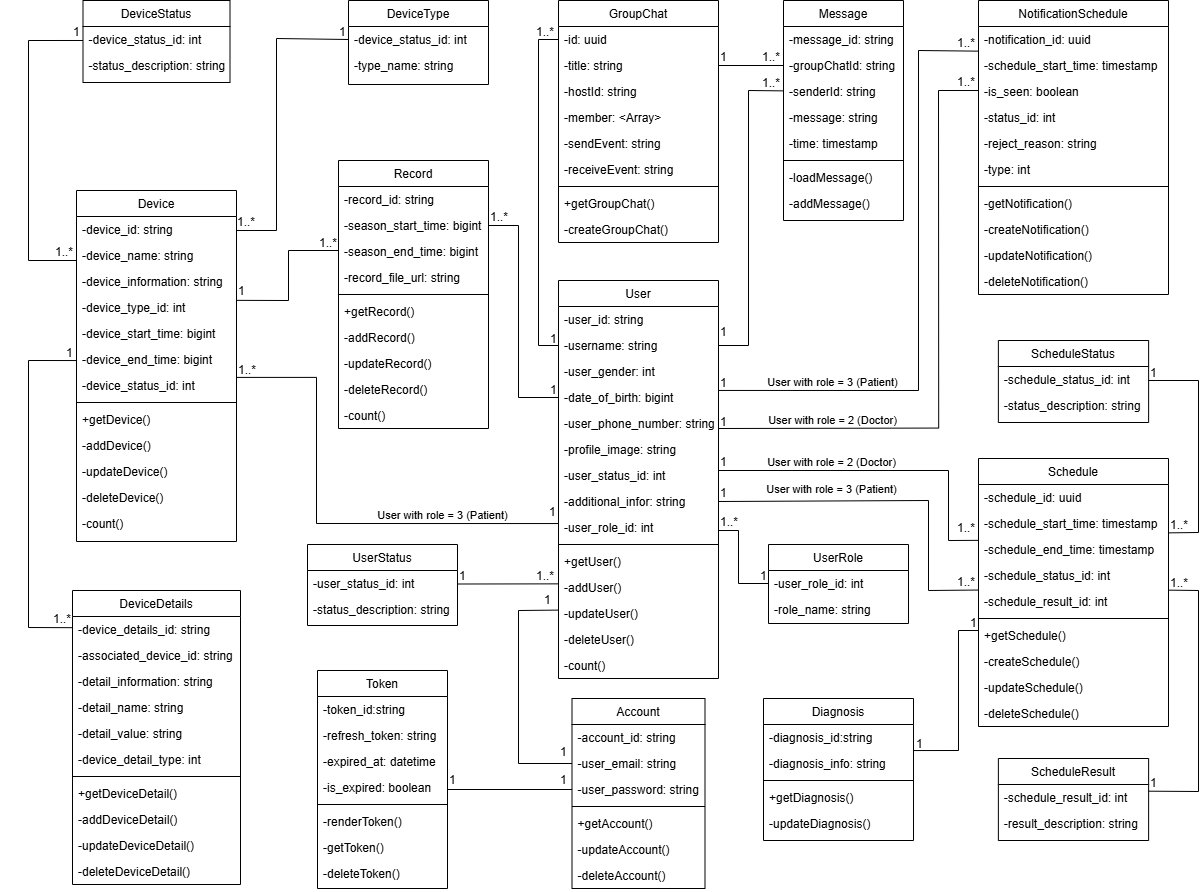
\includegraphics[width=16cm,height=12cm]{Images/system/fmECG_UML.png}
	\caption[Sơ đồ ERD]{\bfseries \fontsize{12pt}{0pt}\selectfont Sơ đồ UML}
	\label{fmECG_UML}
\end{figure}

Hình \ref*{fmECG_UML} thể hiện các lớp trong hệ thống:
\begin{itemize}
	\item Lớp Account (Tài khoản): Chịu trách nhiệm quản lý thông tin cơ bản của tài khoản trong hệ thống. Cung cấp các phương thức để thực hiện thao tác tạo mới, xác thực và quản lý dữ liệu liên quan đến tài khoản người dùng.
	\item Lớp Token: Đảm nhiệm việc lưu trữ và xử lý thông tin về các token sử dụng trong quá trình đăng nhập, đăng ký và xác thực người dùng, đảm bảo tính bảo mật và hiệu quả trong giao tiếp.
	\item Lớp UserRole (Vai trò người dùng): Mô tả và quản lý các vai trò mà người dùng có thể đảm nhiệm, hỗ trợ trong việc phân quyền và xác định hành vi của từng loại vai trò.
	\item Lớp UserStatus (Trạng thái người dùng): Theo dõi và duy trì trạng thái hiện tại của người dùng trong hệ thống, ví dụ như trạng thái hoạt động, bị khóa hoặc đang chờ xác minh.
	\item Lớp User (Người dùng): Lưu trữ thông tin chi tiết của người dùng sau khi đăng ký, cung cấp các phương thức xử lý liên quan đến thông tin cá nhân và các hoạt động của người dùng trong hệ thống.
	\item Lớp DeviceType (Loại thiết bị): Định nghĩa các loại thiết bị khác nhau mà hệ thống hỗ trợ, giúp tổ chức và phân loại thông tin thiết bị một cách khoa học.
	\item Lớp DeviceStatus (Trạng thái thiết bị): Quản lý tình trạng hoạt động của thiết bị, cho phép theo dõi và kiểm soát thiết bị một cách hiệu quả trong hệ thống.
	\item Lớp Device (Thiết bị): Chứa các thông tin cơ bản về thiết bị và người dùng thiết bị, hỗ trợ việc quản lý, tương tác và thu thập dữ liệu từ thiết bị trong hệ thống.
	\item Lớp DeviceDetail (Thông số kỹ thuật): Cung cấp các thông tin kỹ thuật chi tiết về thiết bị, hỗ trợ trong việc cấu hình, kiểm tra và quản lý hiệu năng của thiết bị.
	\item Lớp Record (Dữ liệu phiên đo): Được thiết kế để lưu trữ thông tin về dữ liệu mỗi phiên đo của bệnh nhân, đảm bảo quản lý dữ liệu một cách hiệu quả, an toàn và hỗ trợ xử lý nhanh chóng, chính xác.
	\item Lớp ScheduleType (Loại lịch hẹn): Xác định các loại lịch hẹn trong hệ thống, phục vụ việc phân loại và quản lý lịch hẹn.
	\item Lớp ScheduleStatus (Trạng thái lịch hẹn): Quản lý trạng thái của lịch hẹn (bao gồm các trạng thái như đang chờ xác nhận, đã được bác sĩ chấp nhận, hoặc chưa được xác nhận), giúp theo dõi và cập nhật trạng thái trong suốt vòng đời của lịch hẹn.
	\item Lớp Schedule (Lịch hẹn): Đại diện cho cấu trúc thông tin của một lịch hẹn, cung cấp các phương thức để lưu trữ, truy vấn và xử lý dữ liệu lịch hẹn.
	\item Lớp ConsultationSchedule (Lịch hẹn của bác sĩ): Quản lý các lịch hẹn liên quan đến bác sĩ, hỗ trợ xử lý dữ liệu hiệu quả trong khi vẫn đảm bảo kết nối đồng bộ với thông tin lịch hẹn của bệnh nhân.
	\item Lớp NotificationSchedule (Thông báo liên quan đến lịch hẹn): Chịu trách nhiệm tạo và quản lý các thông báo liên quan đến lịch hẹn, giúp người dùng và bác sĩ cập nhật tình trạng lịch hẹn kịp thời.
	\item Lớp Diagnosis (Chẩn đoán cho bệnh nhân): Quản lý thông tin chẩn đoán bệnh của bệnh nhân (nếu có).
	\item Lớp Message (Tin nhắn): Xử lý thông tin các tin nhắn được gửi trong hệ thống, cho phép người dùng trao đổi thông tin trong các cuộc trò chuyện cá nhân hoặc nhóm.
	\item Lớp GroupChat (Nhóm trò chuyện): Quản lý các nhóm trò chuyện trong hệ thống, cho phép tổ chức và thực hiện các hoạt động giao tiếp nhóm một cách hiệu quả.
\end{itemize}
% \newpage
\subsection{Sơ đồ tuần tự}
% Để phân tích chi tiết hơn từng luồng trong hệ thống thông qua sơ đồ use case và sơ đồ hoạt động, dưới đây là phần thiết kế các sơ đồ tuần tự.

% \subsubsection{Sơ đồ tuần tự đăng ký tài khoản}

% \subsubsection{Sơ đồ tuần tự đăng nhập tài khoản}

% \subsubsection{Sơ đồ tuần tự truy vấn danh sách người dùng}

% \subsubsection{Sơ đồ tuần tự truy vấn danh sách bác sĩ}

% \subsubsection{Sơ đồ tuần tự tìm kiếm người dùng theo ID}

% \subsubsection{Sơ đồ tuần tự truy vấn bệnh nhân theo ID bác sĩ}

% \subsubsection{Sơ đồ tuần tự truy vấn bác sĩ theo ID bệnh nhân}

% \subsubsection{Sơ đồ tuần tự cập nhật thông tin người dùng theo ID}

% \subsubsection{Sơ đồ tuần tự xóa người dùng theo ID}

% \subsubsection{Sơ đồ tuần tự truy vấn danh sách tất cả các thiết bị}

% \subsubsection{Sơ đồ tuần tự tìm kiếm thiết bị theo ID}

% \subsubsection{Sơ đồ tuần tự thêm thiết bị mới}

% \subsubsection{Sơ đồ tuần tự cập nhật thông tin thiết bị theo ID}

% \subsubsection{Sơ đồ tuần tự xóa thiết bị theo ID}

% \subsubsection{Sơ đồ tuần tự thêm thông số kỹ thuật cho thiết bị}

% \subsubsection{Sơ đồ tuần tự điều chỉnh thông số kỹ thuật của thiết bị theo ID}

% \subsubsection{Sơ đồ tuần tự xóa thông số kỹ thuật cho thiết bị theo ID}

% \subsubsection{Sơ đồ tuần tự truy vấn danh sách tất cả các dữ liệu phiên đo}

% \subsubsection{Sơ đồ tuần tự tìm kiếm dữ liệu phiên đo theo ID}

% \subsubsection{Sơ đồ tuần tự tìm kiếm dữ liệu phiên đo theo ID bác sĩ}

% \subsubsection{Sơ đồ tuần tự tìm kiếm dữ liệu phiên đo theo ID bệnh nhân}

% \subsubsection{Sơ đồ tuần tự thêm dữ liệu phiên đo mới}

% \subsubsection{Sơ đồ tuần tự cập nhật thông tin dữ liệu phiên đo dựa trên ID}

% \subsubsection{Sơ đồ tuần tự xóa dữ liệu phiên đo theo ID}

% \subsubsection{Sơ đồ tuần tự truy vấn danh sách toàn bộ lịch hẹn}

% \subsubsection{Sơ đồ tuần tự tìm kiếm lịch hẹn theo ID bệnh nhân}

% \subsubsection{Sơ đồ tuần tự tìm kiếm lịch hẹn theo ID bác sĩ}

% \subsubsection{Sơ đồ tuần tự tạo lịch hẹn mới bởi bệnh nhân}

% \subsubsection{Sơ đồ tuần tự tạo lịch tái hẹn bởi bác sĩ}

% \subsubsection{Sơ đồ tuần tự tìm kiêm các lịch rảnh của bác sĩ theo ID bác sĩ}

% \subsubsection{Sơ đồ tuần tự tìm kiếm danh sách các bác sĩ dựa trên lịch rảnh của bệnh nhân}

% \subsubsection{Sơ đồ tuần tự xác nhận lịch hẹn bệnh nhân đã đặt}

% \subsubsection{Sơ đồ tuần tự xóa lịch hẹn theo ID}

% \subsubsection{Sơ đồ tuần tự thêm chẩn đoán cho bệnh nhân}

% \subsubsection{Sơ đồ tuần tự tìm kiếm chẩn đoán theo ID lịch hẹn}

% \subsubsection{Sơ đồ tuần tự cập nhật thông tin chẩn đoán theo ID lịch hẹn}

% \subsubsection{Sơ đồ tuần tự truy vấn danh sách các thông báo liên quan đến lịch hẹn theo ID người dùng}

% \subsubsection{Sơ đồ tuần tự tạo mới thông báo liên quan đến lịch hẹn}

% \subsubsection{Sơ đồ tuần tự đánh dấu thông báo là đã đọc}

% \subsubsection{Sơ đồ tuần tự xóa thông báo dựa trên ID}

% \subsubsection{Sơ đồ tuần tự truy vấn danh sách tất cả tin nhắn theo ID người dùng}

% \subsubsection{Sơ đồ tuần tự thêm tin nhắn mới}

% \subsubsection{Sơ đồ tuần tự tạo nhóm trò chuyện mới}

% \subsubsection{Sơ đồ tuần tự truy vấn các nhóm trò chuyện theo ID người dùng}

\subsection{Xử lý và phân tích dữ liệu}

Trong phần này, chúng em sẽ xác định và mô tả chi tiết các thực thể cùng các thuộc tính trong hệ thống.
Quá trình này đóng vai trò quan trọng trong việc giúp chúng em hiểu rõ các thành phần cốt lõi, từ đó thiết kế và xây dựng cơ sở dữ liệu một cách tối ưu và hiệu quả.

Trước tiên, chúng em sẽ tiến hành xác định các thực thể trong hệ thống và mô tả chi tiết các thuộc tính của chúng thông qua bảng biểu và sơ đồ liên kết.

\begin{table}[H]
	\raggedright
	\begin{tabularx}{\textwidth}{|p{4.5cm}|X|}
		\hline
		\bfseries Thực thể               & \bfseries Thuộc tính                                                                                           \\ \hline
		Tài khoản                        &
		ID tài khoản, Địa chỉ email, Mật khẩu truy cập                                                                                                                    \\
		\hline
		Token đăng nhập                  &
		ID token, Token làm mới, Hạn sử dụng, Trạng thái token                                                                                    \\
		\hline
		Vai trò người dùng               &
		ID vai trò, Tên vai trò, Mô tả vai trò                                                                                                            \\
		\hline
		Trạng thái người dùng            &
		ID trạng thái, Tên trạng thái, Mô tả trạng thái                                                                                                   \\
		\hline
		Người dùng                       &
		ID người dùng, Tên đầy đủ, Ngày tháng năm sinh, Giới tính, Số liên lạc, Vai trò người dùng, Trạng thái hoạt động, Đường dẫn ảnh đại diện, Thông tin bổ sung \\
		\hline
		Loại thiết bị                    &
		ID loại thiết bị, Tên loại thiết bị, Mô tả loại thiết bị                                                                                          \\
		\hline
		Trạng thái thiết bị              &
		ID trạng thái, Tên trạng thái, Mô tả trạng thái                                                                                                   \\
		\hline
		Thiết bị                         &
		ID thiết bị, Tên thiết bị, Loại thiết bị, Thông tin chi tiết về thiết bị, Tình trạng hiện tại, Ngày bắt đầu thời gian mượn, Ngày kết thúc thời gian mượn                                           \\
		\hline
		Thông số kỹ thuật                &
		ID thông số, Tên thông số, Loại thông số, Giá trị thông số, Mô tả chi tiết thông số                                                                    \\
		\hline
		Dữ liệu phiên đo                 &
		ID dữ liệu phiên đo, Đường dẫn lưu trữ phiên đo, Thời gian bắt đầu thu thập dữ liệu, Thời gian kết thúc thu thập dữ liệu                                          \\
		\hline
		Loại lịch hẹn                    &
		ID loại lịch hẹn, Tên loại lịch hẹn, Mô tả loại lịch hẹn                                                                                          \\
		\hline
		Trạng thái lịch hẹn              &
		ID trạng thái, Tên trạng thái, Mô tả trạng thái                                                                                                   \\
		\hline
		Lịch hẹn                         &
		ID lịch hẹn, Thời gian bắt đầu lịch hẹn, Thời gian kết thúc lịch hẹn, Kết quả lịch hẹn                                                            \\
		\hline
		Lịch hẹn của bác sĩ              &
		ID lịch hẹn của bác sĩ                                                                                                                            \\
		\hline
		Chẩn đoán cho bệnh nhân          &
		ID chẩn đoán, Thông tin chẩn đoán                                                                                                                 \\
		\hline
		Thông báo liên quan đến lịch hẹn &
		ID thông báo, Loại thông báo (gửi cho bác sĩ hoặc gửi cho bệnh nhân), Thời gian bắt đầu lịch hẹn, Nội dung thông báo,
		Trạng thái thông báo (nhắc hẹn, được bác sĩ chấp nhận, đang chờ xác nhận, từ chối, đặt lịch tái khám thành công, bị hủy tự động),
		Trạng thái đã xem, Lý do từ chối lịch (nếu có)                                                                                                    \\
		\hline
		Tin nhắn                         &
		ID tin nhắn, Người gửi tin nhắn, Nhóm trò chuyện nhận tin nhắn, Nội dung tin nhắn, Thời điểm gửi										 \\
		\hline
		Nhóm trò chuyện                  &
		ID nhóm trò chuyện, Tên nhóm trò chuyện, Người tạo nhóm, Danh sách thành viên nhóm, Sự kiện gửi tin nhắn, Sự kiện nhận tin nhắn                             \\
		\hline
	\end{tabularx}
\end{table}

Dựa trên bảng thực thể và thuộc tính đã hoàn thiện, mô hình thực thể liên kết của hệ thống được xác định như sau:

\begin{figure}[H]
	\centering
	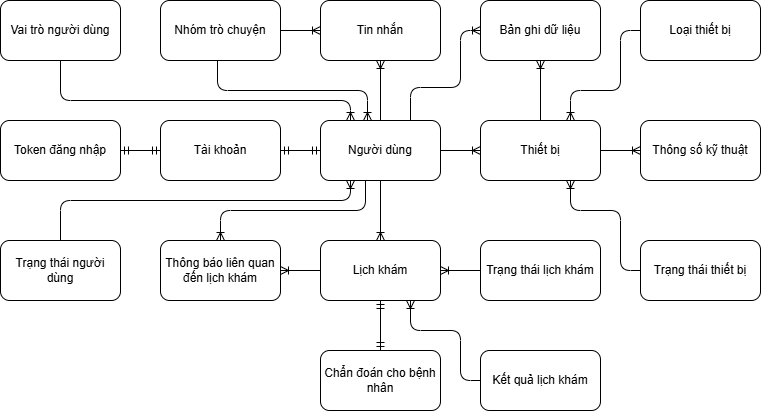
\includegraphics[width=15cm,height=9.5cm]{Images/System/fmECG_connection_entity.png}
	\caption[Mô hình thực thể liên kết]{\bfseries \fontsize{12pt}{0pt}
	\selectfont Mô hình thực thể liên kết}
	\label{entity-diag}
  \end{figure}

\subsection{Kết luận}

Chương này tập trung phân tích tổng quan về hệ thống, nhằm đảm bảo đáp ứng đầy đủ các yêu cầu và mục tiêu đã được đề cập ở các phần trước.

\newpage
